The database schema was designed to ensure structured storage and traceability of all subjective quality evaluation data. Fig.~\ref{fig:db_conceptual} presents the conceptual data model, which defines the main entities and their relationships. The profile entity stores participant metadata, including age, gender, education, ethnicity, country of origin, and device used. The ss\_session entity models individual test sessions and is linked to both the participant profile and the dataset being evaluated. The image entity encodes each image's filename, associated distortion type (distortion\_name), and distortion level (distortion\_level). The test entity stores individual subjective ratings, including the precise timestamp of submission, linked to both the session and the image presented. An auxiliary user\_feedback entity captures optional, anonymous, observer comments and critiques.

The physical implementation of this schema, shown in Fig.~\ref{fig:db_physical}, is realized as a relational database with explicit foreign key constraints to ensure referential integrity. The dataset\_id and profile\_id fields in ss\_session formally enforce the linkage to specific datasets and participants. The test table connects each subjective rating to its session (ss\_session\_id) and image (image\_id), enabling consistent aggregation of ratings into a statistical descriptor such as MOS and confidence intervals per image and per distortion level. The relational model also facilitates efficient querying for downstream statistical analysis and supports reproducibility of the experimental protocol in line with ITU-R BT.500-15 recommendations.

\begin{figure}[htbp]
    \centering
    \begin{subfigure}{0.8\textwidth}
        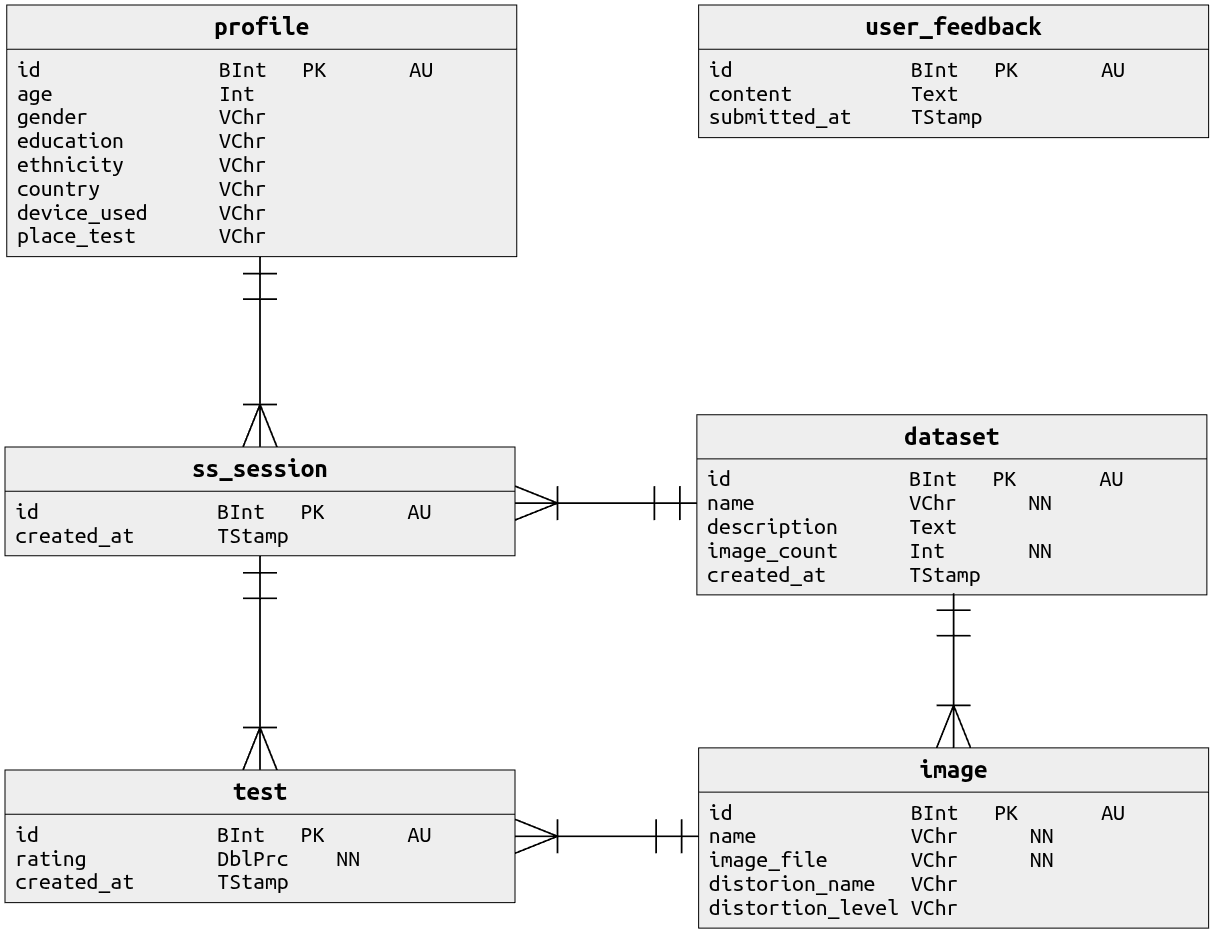
\includegraphics[width=\textwidth]{images/db_conceptual.png}
        \caption{Conceptual database schema showing entity relationships and high-level structure.}\label{fig:db_conceptual}
    \end{subfigure}
    \vfill
    \begin{subfigure}{0.8\textwidth}
        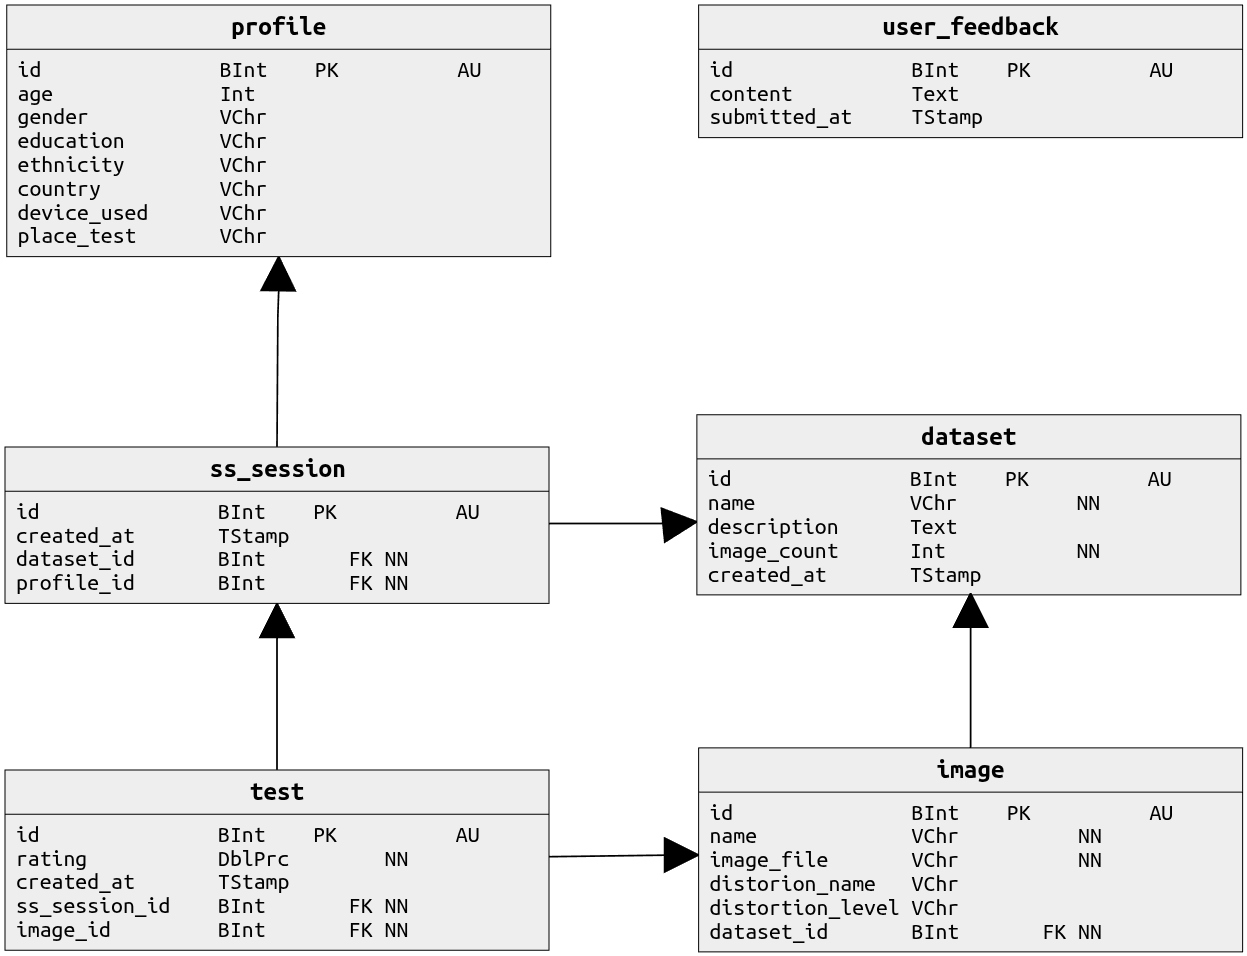
\includegraphics[width=\textwidth]{images/db_physical.png}
        \caption{Physical database schema illustrating actual tables, columns, and implementation details.}\label{fig:db_physical}
    \end{subfigure}
    \caption{Conceptual and physical representations of the database schema.}\label{fig:db_schemas}
\end{figure}

